% This is "sig-alternate.tex" V2.0 May 2012
% This file should be compiled with V2.5 of "sig-alternate.cls" May 2012
%
% This example file demonstrates the use of the 'sig-alternate.cls'
% V2.5 LaTeX2e document class file. It is for those submitting
% articles to ACM Conference Proceedings WHO DO NOT WISH TO
% STRICTLY ADHERE TO THE SIGS (PUBS-BOARD-ENDORSED) STYLE.
% The 'sig-alternate.cls' file will produce a similar-looking,
% albeit, 'tighter' paper resulting in, invariably, fewer pages.
%
% ----------------------------------------------------------------------------------------------------------------
% This .tex file (and associated .cls V2.5) produces:
%       1) The Permission Statement
%       2) The Conference (location) Info information
%       3) The Copyright Line with ACM data
%       4) NO page numbers
%
% as against the acm_proc_article-sp.cls file which
% DOES NOT produce 1) thru' 3) above.
%
% Using 'sig-alternate.cls' you have control, however, from within
% the source .tex file, over both the CopyrightYear
% (defaulted to 200X) and the ACM Copyright Data
% (defaulted to X-XXXXX-XX-X/XX/XX).
% e.g.
% \CopyrightYear{2007} will cause 2007 to appear in the copyright line.
% \crdata{0-12345-67-8/90/12} will cause 0-12345-67-8/90/12 to appear in the copyright line.
%
% ---------------------------------------------------------------------------------------------------------------
% This .tex source is an example which *does* use
% the .bib file (from which the .bbl file % is produced).
% REMEMBER HOWEVER: After having produced the .bbl file,
% and prior to final submission, you *NEED* to 'insert'
% your .bbl file into your source .tex file so as to provide
% ONE 'self-contained' source file.
%
% ================= IF YOU HAVE QUESTIONS =======================
% Questions regarding the SIGS styles, SIGS policies and
% procedures, Conferences etc. should be sent to
% Adrienne Griscti (griscti@acm.org)
%
% Technical questions _only_ to
% Gerald Murray (murray@hq.acm.org)
% ===============================================================
%
% For tracking purposes - this is V2.0 - May 2012

\documentclass{sig-alternate}

\usepackage{listings}
\usepackage{color}

\begin{document}
%
% --- Author Metadata here ---
\conferenceinfo{ICER}{'15 Omaha, Nebraska USA}
%\CopyrightYear{2007} % Allows default copyright year (20XX) to be over-ridden - IF NEED BE.
%\crdata{0-12345-67-8/90/01}  % Allows default copyright data (0-89791-88-6/97/05) to be over-ridden - IF NEED BE.
% --- End of Author Metadata ---

\title{Kennel: Block-based Programming Environment for Python\titlenote{(Produces the permission block, and
copyright information). For use with
SIG-ALTERNATE.CLS. Supported by ACM.}}
\subtitle{[Extended Abstract]
\titlenote{A full version of this paper is available as
\textit{Author's Guide to Preparing ACM SIG Proceedings Using
\LaTeX$2_\epsilon$\ and BibTeX} at
\texttt{www.acm.org/eaddress.htm}}}
%
% You need the command \numberofauthors to handle the 'placement
% and alignment' of the authors beneath the title.
%
% For aesthetic reasons, we recommend 'three authors at a time'
% i.e. three 'name/affiliation blocks' be placed beneath the title.
%
% NOTE: You are NOT restricted in how many 'rows' of
% "name/affiliations" may appear. We just ask that you restrict
% the number of 'columns' to three.
%
% Because of the available 'opening page real-estate'
% we ask you to refrain from putting more than six authors
% (two rows with three columns) beneath the article title.
% More than six makes the first-page appear very cluttered indeed.
%
% Use the \alignauthor commands to handle the names
% and affiliations for an 'aesthetic maximum' of six authors.
% Add names, affiliations, addresses for
% the seventh etc. author(s) as the argument for the
% \additionalauthors command.
% These 'additional authors' will be output/set for you
% without further effort on your part as the last section in
% the body of your article BEFORE References or any Appendices.

\numberofauthors{6} %  in this sample file, there are a *total*
% of EIGHT authors. SIX appear on the 'first-page' (for formatting
% reasons) and the remaining two appear in the \additionalauthors section.
%
\author{
% You can go ahead and credit any number of authors here,
% e.g. one 'row of three' or two rows (consisting of one row of three
% and a second row of one, two or three).
%
% The command \alignauthor (no curly braces needed) should
% precede each author name, affiliation/snail-mail address and
% e-mail address. Additionally, tag each line of
% affiliation/address with \affaddr, and tag the
% e-mail address with \email.
%
% 1st. author
\alignauthor
Austin Cory Bart\\
       \affaddr{Virginia Tech}\\
       \email{acbart@vt.edu}
}
% There's nothing stopping you putting the seventh, eighth, etc.
% author on the opening page (as the 'third row') but we ask,
% for aesthetic reasons that you place these 'additional authors'
% in the \additional authors block, viz.
\date{30 July 1999}
% Just remember to make sure that the TOTAL number of authors
% is the number that will appear on the first page PLUS the
% number that will appear in the \additionalauthors section.

\maketitle
\begin{abstract}

\end{abstract}

% A category with the (minimum) three required fields
\category{H.4}{Information Systems Applications}{Miscellaneous}
%A category including the fourth, optional field follows...
\category{D.2.8}{Software Engineering}{Metrics}[complexity measures, performance measures]

\terms{Theory}

\keywords{ACM proceedings, \LaTeX, text tagging}

\section{Introduction}

The growing awareness of ``Computational Thinking'' as a 21\textsuperscript{st} century competency increasingly requires that computation be positioned in a university's general education curriculum \cite{wing2006computational}.
The long-term vision is that, eventually, Computational Thinking will not be considered as a ``non-major course'' taught by Computer Science.
Instead, it will be solidly embedded within all majors, with well-defined courses on computational biology, computational art, computational psychology, and many others.
These students suffer from low self-efficacy and have poor or inaccurate attitudes towards computing.
For this vision to become a reality, computing educators must introduce Computational Thinking to students with no prior computing experience and motivate them to learn the material.
Critically, instruction must scale with the massive quantities of learners that will be starting with computation.
Even as we desperately train high school teachers to meet the demands of the CS10K projects, universities are demanding computational thinking courses for all their non-CS undergraduates.
Introductory programming environments must therefore
\begin{enumerate}
	\item Motivate learners who have a diverse background and needs.
	\item Support large number of learners with minimal human interaction.
\end{enumerate}

\subsection{Technological Support}

A historically successful approach to gently introducing students to programming is block-based programming, such as Scratch and its successor Snap!.
These environments introduce high-level programming concepts by having students connect blocks representing programming constructs in order to avoid syntactical barriers -- grammatically-incorrect combinations are forbidden by the design of the system.
Although equivalent in computational power, block-based languages have long been known to be unsuitable for professional developers because of their failure to scale and their inflexibilty. 
And yet, instructional design dictates that the learning context should match the performance context as closely as possible to ensure transfer.
Therefore, a recent criticism of this approach is that transferring students from a block-based language to a traditional text-based language is a non-trivial problem that must be studied closely.

Work by Weintrop on the transition from Snap to Python analyzes this transition and offers a number of ways to mediate the transfer through programming tools. 
One of the largest findings is that being able to write inline code inside a Block-based language is extremely helpful to students' learning \cite{Weintrop}.
This idea can be pushed further to allow students to convert their block code to textual form and then translate the textual form back to blocks.
This approach, Mutual Language Translation, is also being explored by Matsuzawa\cite{Matsuzawa} to support the transition from a desktop, block-based programming language to Java in an introductory programming class. 
Although our core approaches are similar, we are looking to develop a browser-based version that supports a motivational programming paradigm with a strong long-term goal towards the development of a mature introductory Python environment that is ideal for novices from external domains.

\subsection{Motivational Support}

In order to identify how students become motivated to learn, we explore the problem from the perspective of the MUSIC Model of Academic Motivation -- despite the name, it is unrelated to music, instead being a meta-theory of motivation developed specifically for motivation in education.
The MUSIC model is a well-supported theory that identifies five key constructs in motivating students \cite{jones-description}:
\begin{description}
	\item[eMpowerment:] The amount of control that a student feels that they have over their learning experience.
	\item[Usefulness:] The expectation of the student that the material they are learning will be valuable to their short-term and long-term goals.
	\item[Success:] The student's belief in their own ability to complete their work.
	\item[Interest:] The student's perception of how the assignment appeals to situational or dispositional interests.
	\item[Caring:] The students perception of their professor's and classmates attitudes toward them.
\end{description}
The premise of the MUSIC model is that one or more of these constructs must be sufficiently activated in order for a student to be intrinsically motivated, which increases their chances of succeeding.
Learners are individuals with their own predispositions and drives -- it is unlikely that motivational pedagogies can be one-size fit all.

Over the past few years, there have been many potential motivating contexts explored for introductory Computer Science courses, such as game development or mobile application design. 
Most of these contexts rely on an expectation of interest, without providing a compelling case for authentic usefulness -- most students don't expect to become game designers, for instance, but simply enjoy playing games.
One of the more popular methods that falls into this area is Media Computation, where students learn programming through audio and image manipulation. 
Although wildly deployed, a review of these curricular materials by Guzdial \cite{guzdial2006imagineering} in light of Situated Learning Theory found that 1) students did not find this an authentic context, and 2) intense rhetoric was insufficient to convince them that it was authentic. 
Guzdial leaves open the question of what contexts can be truly authentic for non-majors, given the relative novelty of Computational Thinking.

\section{Approach}

\begin{figure*}
\label{fig-full-kennel}
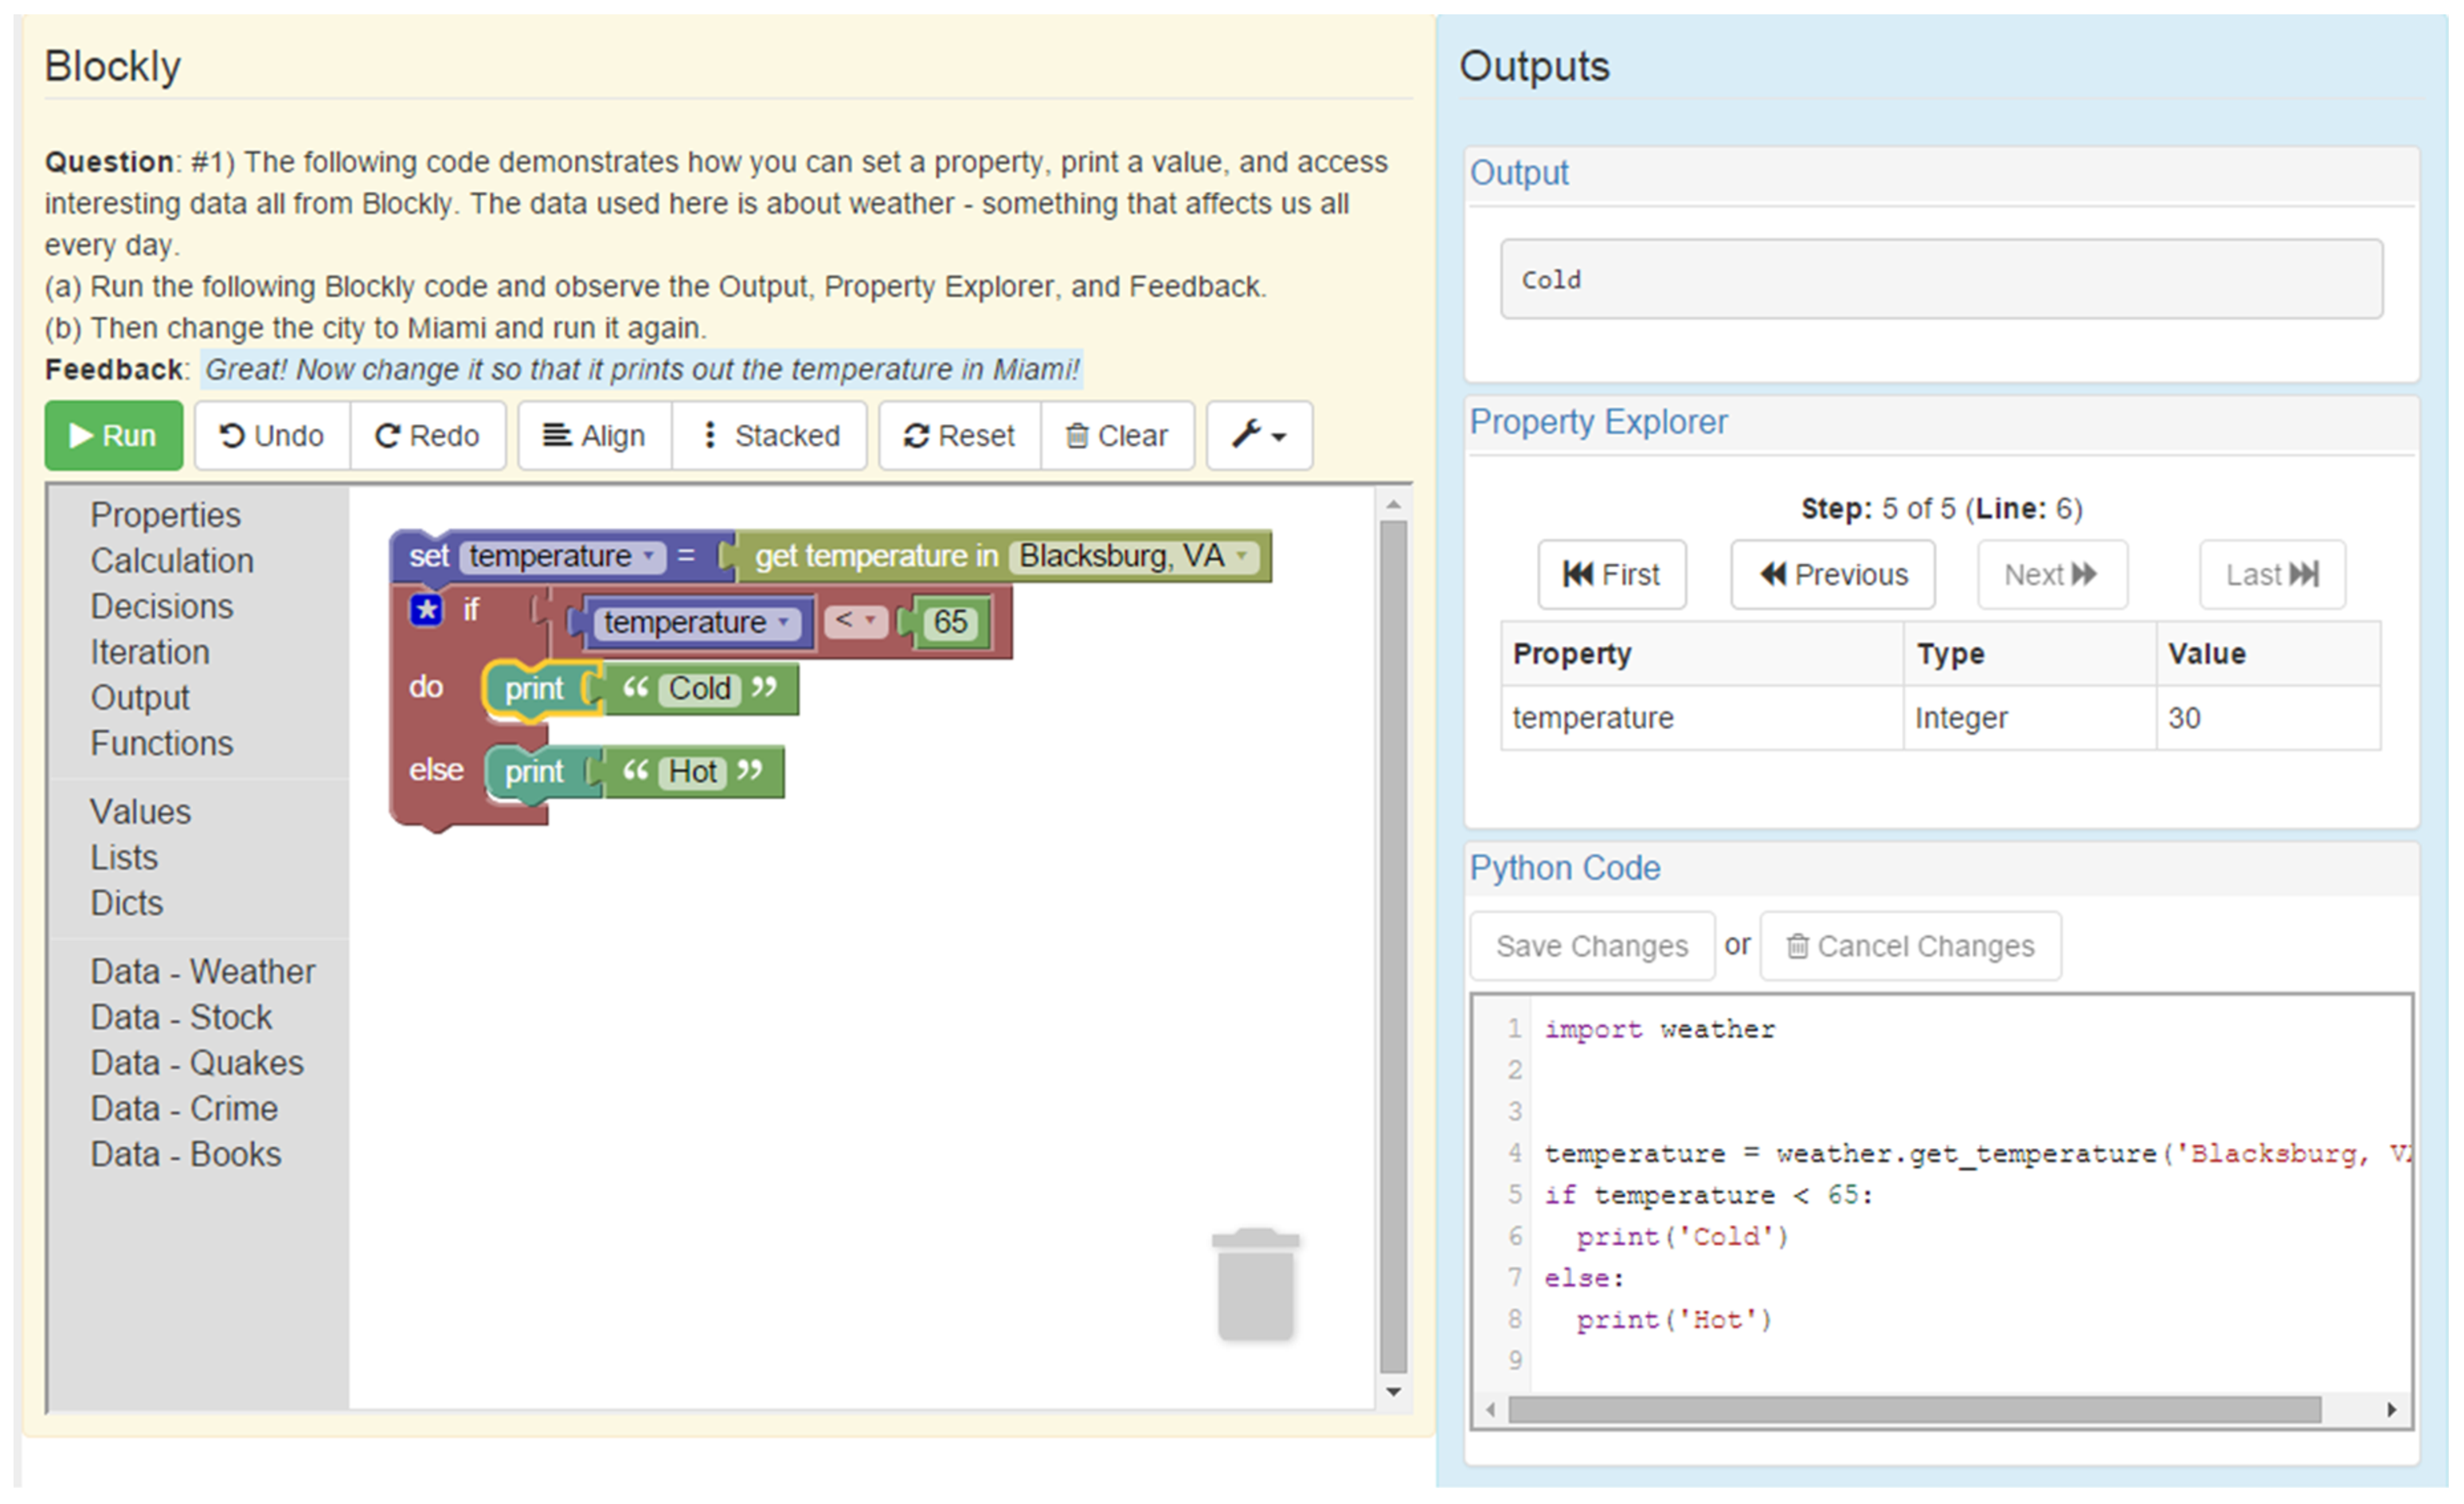
\epsfig{file=images/full-kennel.eps, width=\linewidth}
\caption{A full view of an embedded Kennel problem.}
\end{figure*}

We submit big data as an answer to teach Computer Science and Computational Thinking, separating the material into context and content.
Big data provides an authentic, useful context for both kinds of students, since using it is something that almost all fields are beginning to find relevant.
Additionally, it is readily possible to find data sources that connect to the world around the student and their past experiences, establishing a sense of personalized interest.
When students inevitably ask, ``What am I going to be using this for?'', it is possible to point to well-defined  big data problems in their field requiring computation; the rhetroic is still needed, since the students are still novices, but there is no necessity to lie or exaggerate the usefulness \cite{guzdial2006imagineering}.


Python is a popular choice for introductory programming because it  has a lightweight syntax [Guo paper]


Research questions:

How can the system promote transfer

How to create a motivating programming environment

How do students use the block-based programming environment

Situated Learning, authentic learning through big data.

Support constructivist problems and more typical problems

Mastery learning to encourage multiple attempts

The block-based environment directly supports the core features of course by only exposing the subset of python that supports the material. In our model of computational thinking:
\begin{itemize}
	\item Abstraction is the method by which real-world entities are encoded in a computer, according to a stakeholder's context.
	\item Decisions allow programs
	\item Iteration
\end{itemize}

There are many limitations to the particular model of Computational Thinking used in this course, and a full discussion of its merits are outside the scope of this paper. We refer the reader to [Kafura citation] for a complete description of the course. Instead, we focus on how the design of the programming model can support the pedagogical goals of the course.

\section{Kennel}

In this section of the paper, we introduce our new online programming environment named Kennel.
The goal of Kennel is to be a beginner-friendly programming environment that scaffolds the learner into maturity while supporting a number of theory-driven, pedagogical objectives.
Internally, Kennel uses a modified version of the open-source Blockly library to handle the block editor, a modified version of the open-source Skulpt library to execute python code, and an unmodified version of the open-source CodeMirror library to handle the text editor.
The system promotes the transfer process by supporting Mutual Language Transformation between Blockly and Python -- at any time, code can be transferred back-and-forth between the block editor and the text editor.
This transfer is highly optimized so that there is no usability delay in observing the differences between blocks and text.

The Skulpt execution environment resides entirely within the users' browser, so there is no reliance on an external server. This includes a built-in, client-side Property Explorer to support program and data visualization. This execution environment supports a large number of native Python libraries, including custom ones developed for Big Data analysis. The long-term goal of this project is to support a useful set of rich libraries so that sophisticated applications can be developed -- going beyond traditional console-based problems. In this sense, the project is similar to other Skulpt-based environments such as Pythy and CodeSkulptor. However, Kennel seeks to maintain 100\% compatibility with existing Python APIs so that all code written is authentic.

Kennel is not just a code-authoring environment but also a system for guided practice. Instructors can create problems with interactive feedback. As students complete and struggle with milestones within the problem, they can be given just-in-time feedback, support, and encouragement. As they complete problems, this data can be reported to an interested central location, suitable for grading and course completion information. The system also tracks a number of events and user interactions for fine-grained analysis.

\subsection{Mutual Language Translation}

\begin{figure}
\label{fig-mlt-overview}
\psfig{file=images/graphics.ps, width=\linewidth}
\caption{The flow of code in the Mutual Language Translation system}
\end{figure}

The largest novel technical contribution of this project is the Mutual Language Translation between Blockly and Python.
Figure \ref{fig-mlt-overview} gives an overview of the flow of code in the environment, and figures \ref{fig-example-blockly} and \ref{fig-example-python} demonstrate the near-equivalency of the output of the two code editors.
Blockly outputs valid python source code, which can be passed into Skulpt in order to retrieve a JSON representation of the Abstract Syntax Tree.
Alternatively, the Python source of the Skulpt program can be edited directly by the user. 
Either way, this AST is parsed using our Py2Block library in order to generate an XML representation that Blockly can transform into its blocks.

Blockly already supports compilation of its blocks to Python, JavaScript, and Dart.
However, this multiple language support comes at a cost of reduced isomorphism - each language has different syntax for their common operations, and it is impossible to create a fully-featured block language with a one-to-one mapping between them.
For example, JavaScript has no support for parallel assignment, a commonly-used feature in Python, while Python does not have increment or decrement operators.

Instead of trying to satisfy multiple languages, we have dropped support for JavaScript in favor of a more full-featured mapping to Python.
Most of the changes are minor details that introduce pythonic syntax details: functions blocks are labeled ``define'', assignment blocks have an ``='' operator, the ``add item to list'' block is renamed to ``append''.
Blockly has been extended with new language features to include support for creating and retrieving dictionaries.
Globals - not useful in a CS course, students shouldn't write functions that affect global scope

Eventually, the interface should offer a complete isomorphic mapping to Python - however, there are a number of complications to resolve before that can occur.
For instance, Python uses square brackets for both list indexing and dictionary access.
There is a strong desire to differentiate between these distinctive types of access, visible in the block view as two distinct kinds of blocks (``get ith element of list'' vs. ``get key from dict'' blocks).
However, depending on what features of python are supported, it can be difficult or even impossible to statically identify the usage of a given pair of brackets -- instead, dynamic analysis needs to be combined with abstract interpretation techniques, such as those used in PySonar .  %TODO: CITE
Typically these systems suffer from state explosion due to the large number of metaprogramming techniques usable in a python programmer - however, they are uniquely suitable for an educational environment due to the reduced subset of Python needed in practice by beginners.

A less technical and more user-oriented question is how many language details should be exposed, and what rate.
A rarely used feature of ``for'' loops in Python is to contain an ``else'' clause that is executed upon successful completion of the loop (that is, when it is not prematurely escaped using a ``break'' statement).
This advanced language feature is meant to draw special attention to connected actions that must be performed after the iteration is completed.
If an ``else'' clause were made available to beginners first trying to grapple with iteration, it is likely they would confuse the concept with the conditional ``else'' clause used in ``if'' statements.
Cognitive Load Theory can be a harsh mistress for beginners, and the user interface needs to avoid exposing unnecessary details where possible.
It can be very difficult to recognize when the learner is ready to understand parallel assignment, and therefore able to specify multiple variables on the left side of an assignment block.
This is actually an advantage of traditional text-based environments, since they hide all advanced features by their very nature.
	
\subsection{Data Science Blocks}

In accordance with our motivational theory, we seek to move past interest-based programming into broadly useful programming contexts.
To that end, we use Data Science as an authentic context for teaching introductory computing.
As previously mentioned, Skulpt supports a number of Python APIs, and it can also be extended with any existing pure-python libraries or JavaScript libraries that use the Skulpt API.
We use a fork of Skulpt with partially equivalent implementations for the popular MatPlotlib library (TODO: cite waywaard) and also extended it with our own implementation of the CORGIS project.
The Waywaard MatPlotLib API provides a ``plot(list)'' function to create simple line plots.
By basing everything around the MatPlotLib API, students can seamlessly shift to a serious programming environment without loss of code or productivity. 

The CORGIS (Collection of Real-time, Giant, Interesting Datasets) project strives to make it trivial to bring Big Data into introductory programming courses through carefully scaffolded libraries -- including rapidly changing high velocity data (e.g., weather, stocks) or massive high volume datasets (e.g., census and crime report data).
These libraries are pure python, and are rapidly integrated into Skulpt and exposed through the block editor, as seen in figure \ref{fig-example-blockly}.
Data returned from their interface is extremely simple -- usually either primitive (numbers and text) or simply structured (heterogenous dictionaries and homogenous lists), ensuring that students can begin working with Big Data blocks at the earliest possible point in the course.

During the course, students take advantage of the internal caching mechanism of the CORGIS libraries to work on recorded data.
This simplifies the debugging process since programs perform predictably and are no longer dependent on external data services.
When students are ready to run their programs against live data, they can move offline to a traditional programming environment and run in regular production.
This caching mechanism also benefits from an assessment view - a students program can be checked for robustness by invisibly changing the values returned by the big data functions.

\begin{figure*}[ht]
\centering
\begin{minipage}[b]{0.45\linewidth}
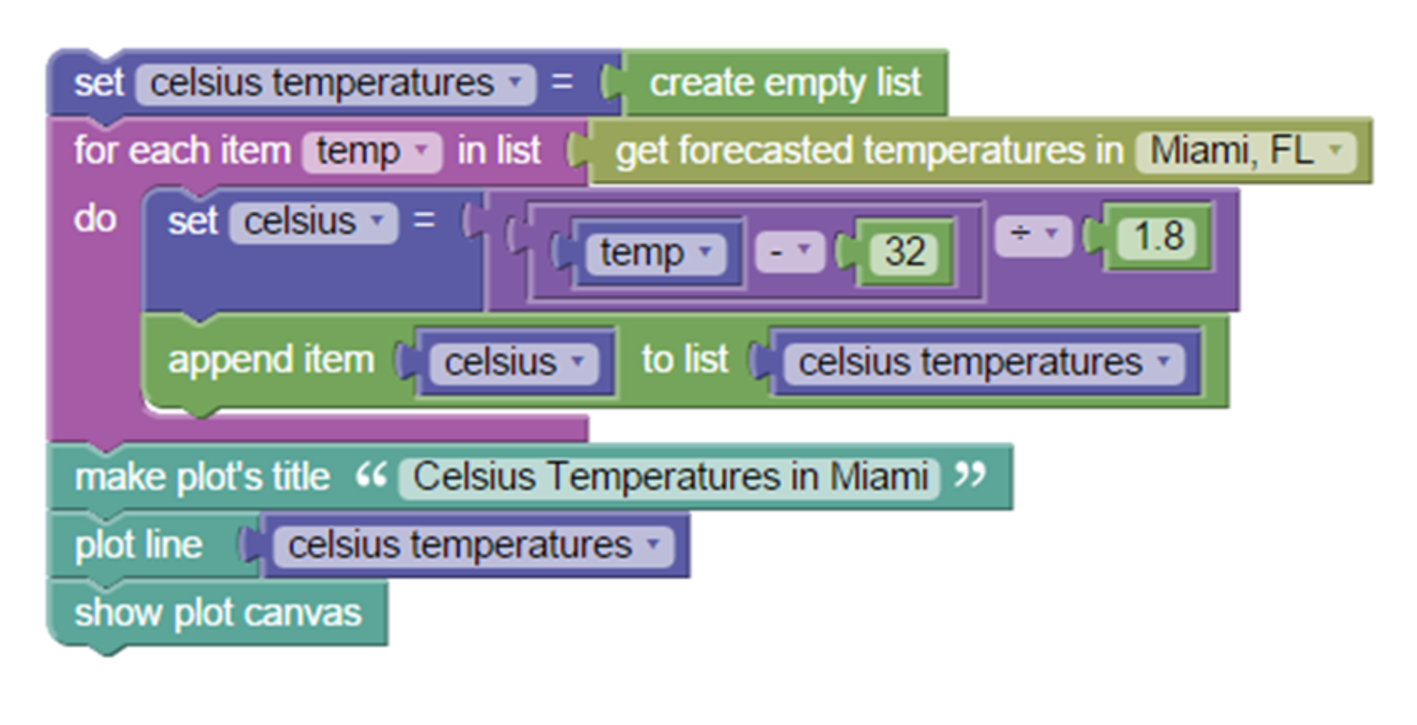
\psfig{file=images/blockly-example.eps, width=\linewidth}
\caption{Blockly Code}
\label{fig-example-blockly}
\end{minipage}
\quad
\begin{minipage}[b]{0.45\linewidth}
\definecolor{mymauve}{rgb}{0.58,0,0.82}
\lstset{stringstyle=\color{mymauve}}
\begin{lstlisting}[language=Python, showstringspaces=false, columns=fullflexible]
import weather
import matplotlib.pyplot as plt

celsius_temperatures = []
for t in weather.get_forecasts('Miami, FL'):
  celsius = (t - 32) / 1.8
  celsius_temperatures.append(celsius)
plt.title('Celsius Temperatures in Miami')
plt.plot(celsius_temperatures)
plt.show()
\end{lstlisting}
\caption{Python Code}
\label{fig-example-python}
\end{minipage}
\end{figure*}


Eventually, more sophisticated visualizations will be required.
Users are often highly motivated to create user interfaces to control their software interactively.
By supporting a GUI library like TKinter or PyQT, students could construct an entire python program in the browser, and then immediately share their work with friends, families, and potentially even colleagues.
This overcomes a limitation of traditional python development - python code can only be run in a Python interpreter with the appropriate libraries, and most end-users do not have such software already installed.
Once relevant libraries are added to our Skulpt fork, students can create and share sophisticated programming projects seamlessly.
	
\subsection{Guided Problems}

A limitation of programming environments like Snap! is that they are not meant to be pedagogically interactive - students completing an assignment in the system are not guided to success.

One of the most powerful features of Kennel is the interactive feedback feature. Every time that students run their code, it is checked against instructor-provided logic. If the students code fails for some reason, they are offered a suggestion or motivational remark.

This section will discuss the technical infrastructure for these, the kinds of problems they support, and the pedagogical advantages of this for large-scale classrooms.

	Constraints -> strings
	
	In order to manage class sizes, automatic feedback systems can be tremendously useful.
	
	Some curriculums teach functions first
	
	We can simulate unit testing by manipulating the outputs of our big-data functions, so that the students code can
 be tested against multiple inputs.
	
\subsection{Persistence and Event Tracking}

In our pilot of Kennel, the system is embedded within an online, interactive textbook based off the popular Runestone platform. % Cite runestone
All work completed by the student is reported to the system in order to assign course credit.
Additionally, in-progress development is persisted on the server using a fault-tolerant caching mechanism.
\begin{enumerate}
  \item User triggers a change \textit{Or} Client reloads page, and an entry is found in the LocalStorage.
	\item Change is stored in LocalStorage.
	\item Change is sent to server.
  \item Server successfully stores change \textit{Or} Fails to store the change.
	\item Upon receipt of successful change, the Client clears entry in LocalStorage \textit{Or} It never recieves the receipt and instead keeps the entry until a page reload.
\end{enumerate}
Finally, all student interactions with the systems' user interface are tracked for logging purposes.
This includes students program edits, down to nearly the key-stroke level.
These can be used in order to build up a complete representation of the students code as they develop.
	
\subsection{Teacher Tools}

This section will talk about the teacher-side tools that we've developed and how they can be used in a classroom environment.

Real-time dashboard of events as students perform them

Debugging errors in questions in real-time.

Monitoring struggling students in order to approach them rather than just letting them bash their heads in.
	
\subsection{Property Explorer}

The dominant algorithm visualization software in online python execution is CodeLens

- server

- slow, requires internet

- introduces some complexity - frames and object model

Debugging student's state

Property Explorer

	Aligns blockly blocks to lines of python
	
	Renders python data type, value
	
	Future: render origin of property


\subsection{Missing features}

One of the biggest missing features of Blockly that has not been rectified is object-oriented classes. Although Skulpt supports this, we need blocks for it.

A number of other minor language features are also unsupported, such as tuples, pattern matched assignments, and while loops.

Figure \ref{fig-blockly-custom} demonstrates how Blockly can support arbitrary code execution through the Code Block, Code Expression, and user-defined Function blocks.

Describe how these can also be used to transition students to block-based programming (reference Weintrop).

\begin{figure}
\label{fig-blockly-custom}
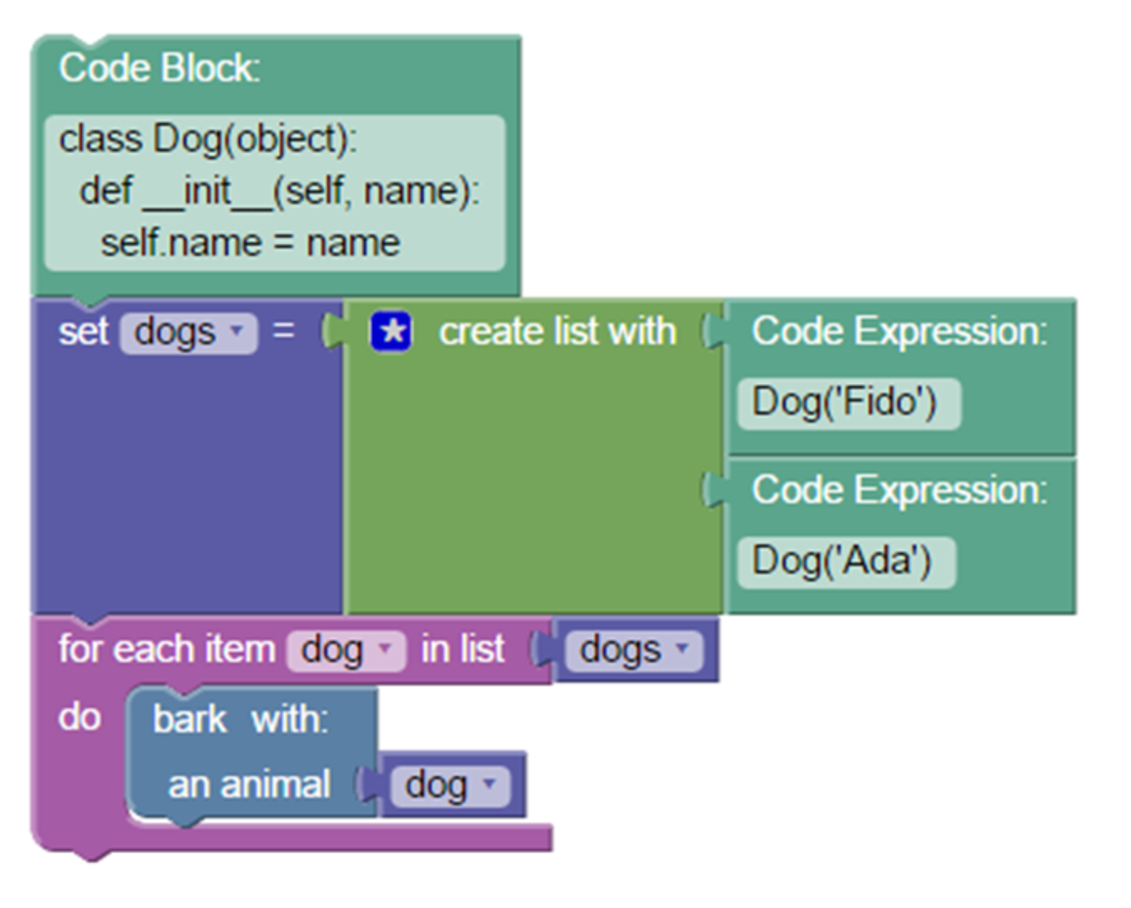
\psfig{file=images/blockly-custom.eps, width=\linewidth}
\caption{Missing language features can be used through the Code Block, Code Expression, and user-defined Function blocks}
\end{figure}


\section{Metholodology}

The research questions in this paper ask how the design of this new block-based language can support the learning process of non-majors. To that end, we conducted a semester-long study of its use in a new Computational Thinking course.

The participants in the study were students in the undergraduate computational thinking class. These are 40 non-majors from X different majors. This was the second time this course was offered. 
The survey instrument was designed around the MUSIC Model of Academic Motivation's core components. 
The self-report, non-anonymous survey had a respondent rate of 83%. 
Surveys were conducted at the start of the course, midway through the course after they completed the Blockly unit, and at the end of the course after they completed the Python unit.
The primary data collector was the assistant instructor for the course and regularly interacted with the students. 

There were two instructors and three teaching assistants - one of the teaching assistants was sophomore level computer science major, and the other two were former students of the class (one in international studies and the other in civil engineering). 

We collected fine-grained interaction data over the course of the Blockly section of the course and then matched that with self-reported, non-anonymous surveys designed to measure students motivation during the semester.
Graphs of student submissions

\section{Data and Conclusions}

There were far fewer non-run events than were expected. This suggests that beginners were unable to engage with our Property Explorer. It is not as simple as giving them a tool.

Almost no conversions - students were not trying to write Python code in the browser.

Blockly and Python had a similar level of perceived usefulness

Student subverted the automatic checker

Tools do not replace instruction - students did not 

Was useful for identifying errors in problems early

Was useful in keeping the classroom manageable.

Some students reported the motivating remarks helpful, some reported them to be boring.

Some students felt that blockly took too long, some felt it wasn't long enough.

\section{Future Work}

Social sharing

full application development with Tkinter similar to CodeSkulptor. CodeSkulptor features its own API named SimpleGUI that is meant to be similar but distinct from TKinter, PIL, and Pygame \cite{Tang}. Unfortunately, this means that code cannot be transferred as a project matures, and existing TKinter examples cannot be used in the browser.

more sophisticated data analysis - more visualizations, free form data integration

Although the current user interface places a strong emphasis on the block-based programming, this isn't necessary - future versions will offer an alternative view with emphasis on the textual programming. By promoting the text authoring screen to the primary region of screen real-estate, the mental model of the learner should be affected.

What order do we show blocks?

Can we model students' frustration, can we make the system more friendly? Suggest when they should take a break?


%
% The following two commands are all you need in the
% initial runs of your .tex file to
% produce the bibliography for the citations in your paper.
\bibliographystyle{abbrv}
\bibliography{sigproc}  % sigproc.bib is the name of the Bibliography in this case
% You must have a proper ".bib" file
%  and remember to run:
% latex bibtex latex latex
% to resolve all references
%
% ACM needs 'a single self-contained file'!
%
%APPENDICES are optional
%\balancecolumns
\appendix
%Appendix A
\subsection{References}
Generated by bibtex from your ~.bib file.  Run latex,
then bibtex, then latex twice (to resolve references)
to create the ~.bbl file.  Insert that ~.bbl file into
the .tex source file and comment out
the command \texttt{{\char'134}thebibliography}.
% This next section command marks the start of
% Appendix B, and does not continue the present hierarchy
\section{More Help for the Hardy}
The sig-alternate.cls file itself is chock-full of succinct
and helpful comments.  If you consider yourself a moderately
experienced to expert user of \LaTeX, you may find reading
it useful but please remember not to change it.
%\balancecolumns % GM June 2007
% That's all folks!
\end{document}
